% ============================================================
%  On the Closed-Form of Flow Matching — 15-min presentation
%  Beaudouin & Collin  |  Master MVA, ENS Paris-Saclay
%  Generative Modeling 2025-2026
% ============================================================
\documentclass[10pt,aspectratio=169]{beamer}

% ────────────────────────────────────────────────────────────
%  PACKAGES
% ────────────────────────────────────────────────────────────
\usepackage[T1]{fontenc}
\usepackage[utf8]{inputenc}
\usepackage[english]{babel}
\usepackage{amsmath,amssymb,amsfonts,mathtools,bm}
\usepackage{graphicx}
\usepackage{booktabs}
\usepackage{multirow}
\usepackage{array}
\usepackage{tikz}
\usetikzlibrary{arrows.meta,positioning,shapes.geometric,
                decorations.pathmorphing,calc,fit,backgrounds}
\usepackage[most]{tcolorbox}
\usepackage{appendixnumberbeamer}
\usepackage{microtype}
\usepackage{xcolor}
\graphicspath{{figs/}}

% ────────────────────────────────────────────────────────────
%  COLOURS  (matching the report)
% ────────────────────────────────────────────────────────────
\definecolor{TitleColor}{HTML}{102A43}
\definecolor{AccentColor}{HTML}{2F80ED}
\definecolor{SoftBlue}{HTML}{EAF2FF}
\definecolor{SoftGray}{HTML}{F7F9FC}
\definecolor{TextGray}{HTML}{3A3A3A}
\definecolor{LightAccent}{HTML}{90C4F9}
\definecolor{DarkAccent}{HTML}{1A5FA8}
\definecolor{GreenOK}{HTML}{219653}
\definecolor{RedKO}{HTML}{EB5757}
\definecolor{Orange}{HTML}{F2994A}

% ────────────────────────────────────────────────────────────
%  BEAMER THEME
% ────────────────────────────────────────────────────────────
\usetheme{default}
\setbeamertemplate{navigation symbols}{}

\setbeamercolor{background canvas}{bg=white}
\setbeamercolor{frametitle}{fg=TitleColor, bg=SoftBlue}
\setbeamerfont{frametitle}{series=\bfseries, size=\large}
\setbeamerfont{framesubtitle}{size=\small, series=\normalfont}

\setbeamercolor{title}{fg=white}
\setbeamercolor{subtitle}{fg=LightAccent}
\setbeamercolor{author}{fg=white}
\setbeamercolor{institute}{fg=LightAccent}
\setbeamercolor{date}{fg=LightAccent}

\setbeamercolor{itemize item}{fg=AccentColor}
\setbeamercolor{itemize subitem}{fg=DarkAccent}
\setbeamertemplate{itemize item}{\textcolor{AccentColor}{\small$\blacktriangleright$}}
\setbeamertemplate{itemize subitem}{\textcolor{DarkAccent}{\footnotesize$\bullet$}}
\setbeamertemplate{enumerate item}{%
  \textcolor{AccentColor}{\bfseries\insertenumlabel.}}

\setbeamercolor{block title}{fg=white, bg=TitleColor}
\setbeamercolor{block body}{fg=TextGray, bg=SoftBlue}
\setbeamercolor{block title alerted}{fg=white, bg=RedKO}
\setbeamercolor{block body alerted}{fg=TextGray, bg=RedKO!8}
\setbeamercolor{block title example}{fg=white, bg=GreenOK}
\setbeamercolor{block body example}{fg=TextGray, bg=GreenOK!8}

%  footline
\setbeamertemplate{footline}{%
  \begin{beamercolorbox}[wd=\paperwidth,ht=2.2ex,dp=0.8ex,
      leftskip=1em,rightskip=1em]{structure}%
    \textcolor{TextGray!70}{\scriptsize
      Beaudouin \& Collin \;--\; On the Closed-Form of Flow Matching
      \hfill
      \textcolor{AccentColor}{\insertframenumber\,/\,\inserttotalframenumber}}
  \end{beamercolorbox}%
}

%  frame title with blue rule
\setbeamertemplate{frametitle}{%
  \nointerlineskip
  \begin{beamercolorbox}[wd=\paperwidth,
      leftskip=0.8em,rightskip=0.8em,sep=0.4em]{frametitle}
    \usebeamerfont{frametitle}\insertframetitle
    \ifx\insertframesubtitle\@empty\else
      \hspace{0.5em}\textcolor{AccentColor!80}{\normalsize|}\hspace{0.3em}%
      \usebeamerfont{framesubtitle}\textcolor{DarkAccent}{\insertframesubtitle}
    \fi
  \end{beamercolorbox}
  \begin{beamercolorbox}[wd=\paperwidth,ht=1.5pt,dp=0pt]{}
    \color{AccentColor}\rule{\paperwidth}{1.5pt}
  \end{beamercolorbox}%
}

%  title page
\defbeamertemplate*{title page}{custom}{%
  
\begin{tikzpicture}[remember picture, overlay]
    \fill[TitleColor] (current page.north west) rectangle (current page.south east);
    \fill[AccentColor!18!TitleColor]
      (current page.south west) rectangle +(\paperwidth, 0.09\paperheight);
    \foreach \k in {1,...,6}{%
      \draw[white, opacity=0.04+0.025*\k, line width=1.2pt]
        ($(current page.north east)+(-\k*1.2cm,0)$) --
        ($(current page.south east)+(-\k*1.2cm,0)$);}
    \foreach \a in {15,55,...,335}{%
      \fill[AccentColor, opacity=0.12]
        ($(current page.center)+({\a}:8cm)$) circle (1.8pt);}
  \end{tikzpicture}
  \vspace{1.1cm}
  \hspace{0.7cm}%
  \begin{minipage}{0.86\paperwidth}
    {\LARGE\bfseries\color{white}\inserttitle}\\[0.28em]
    {\large\color{LightAccent}\insertsubtitle}\\[1.2em]
    {\normalsize\color{white!85!TitleColor}\insertauthor}\\[0.22em]
    {\small\color{LightAccent}\insertinstitute}\\[0.18em]
    {\small\color{LightAccent!70}\insertdate}
  \end{minipage}%
}

% ────────────────────────────────────────────────────────────
%  CUSTOM BOXES
% ────────────────────────────────────────────────────────────
\newtcolorbox{hlbox}[1][]{enhanced,
  colback=SoftBlue, colframe=AccentColor,
  boxrule=0.8pt, arc=3pt,
  left=5pt,right=5pt,top=3pt,bottom=3pt,
  fonttitle=\bfseries\small\color{TitleColor}, #1}

\newtcolorbox{resbox}[1][]{enhanced,
  colback=GreenOK!8, colframe=GreenOK,
  boxrule=0.8pt, arc=3pt,
  left=5pt,right=5pt,top=3pt,bottom=3pt,
  fonttitle=\bfseries\small\color{GreenOK!60!black}, #1}

\newtcolorbox{keybox}[1][]{enhanced,
  colback=TitleColor!6, colframe=TitleColor,
  boxrule=0.8pt, arc=3pt,
  left=5pt,right=5pt,top=3pt,bottom=3pt,
  fonttitle=\bfseries\small\color{white},
  attach boxed title to top left={yshift=-1.8mm,xshift=4mm},
  boxed title style={colback=TitleColor,arc=2pt,boxrule=0pt}, #1}

\newtcolorbox{warnbox}[1][]{enhanced,
  colback=Orange!10, colframe=Orange,
  boxrule=0.8pt, arc=3pt,
  left=5pt,right=5pt,top=3pt,bottom=3pt, #1}

% ────────────────────────────────────────────────────────────
%  MATH COMMANDS
% ────────────────────────────────────────────────────────────
\newcommand{\R}{\mathbb{R}}
\newcommand{\E}{\mathbb{E}}
\newcommand{\cN}{\mathcal{N}}
\newcommand{\cL}{\mathcal{L}}
\newcommand{\dd}{\mathrm{d}}
\newcommand{\norm}[1]{\left\lVert #1 \right\rVert}
\newcommand{\Id}{\mathrm{Id}}

% ============================================================
%  DOCUMENT
% ============================================================
\begin{document}

\title{On the Closed-Form of Flow Matching}
\subtitle{Generalization Does Not Arise from Target Stochasticity}
\author{Gaspard Beaudouin \quad \& \quad Yentl Collin}
\institute{Master MVA, {\'E}cole Normale Sup{\'e}rieure Paris-Saclay}
\date{Generative Modeling --- 2025--2026}

{\setbeamertemplate{footline}{}
\begin{frame}[plain]
  \usebeamertemplate{title page}
\end{frame}}
\addtocounter{framenumber}{-1}

% ────────────────────────────────────────────────────────────
%  OUTLINE
% ────────────────────────────────────────────────────────────
\begin{frame}{Outline}
  \begin{columns}[t]
    \begin{column}{0.46\textwidth}
      \textcolor{TitleColor}{\textbf{\large Theory}}
      \bigskip

      \begin{enumerate}
        \item[\textcolor{AccentColor}{\bfseries 1.}] Motivation \& Central Question
        \item[\textcolor{AccentColor}{\bfseries 2.}] Background: Diffusion \& Flow Matching
        \item[\textcolor{AccentColor}{\bfseries 3.}] FM--Diffusion Equivalence
        \item[\textcolor{AccentColor}{\bfseries 4.}] Closed-Form Optimal Velocity \& Collapse
      \end{enumerate}
    \end{column}
    \begin{column}{0.50\textwidth}
      \textcolor{TitleColor}{\textbf{\large Experiments}}
      \bigskip

      \begin{enumerate}
        \item[\textcolor{AccentColor}{\bfseries 5.}] Stochasticity Analysis (Fig.~1)
        \item[\textcolor{AccentColor}{\bfseries 6.}] Velocity Approximation Failure (Fig.~2)
        \item[\textcolor{AccentColor}{\bfseries 7.}] Generalization Switching Time (Fig.~3)
        \item[\textcolor{AccentColor}{\bfseries 8.}] Beyond the Paper: Ablations
        \item[\textcolor{AccentColor}{\bfseries 9.}] EFM on Fashion-MNIST
        \item[\textcolor{AccentColor}{\bfseries 10.}] Discussion \& Conclusion
      \end{enumerate}
      \vspace{0.6em}
      \begin{hlbox}
        \small\textbf{Paper:} Bertrand, Gagneux, Massias, Emonet.
        \textit{NeurIPS 2025.}
      \end{hlbox}
    \end{column}
  \end{columns}
\end{frame}

% ============================================================
\section{Motivation}
% ============================================================
\begin{frame}{The Central Puzzle}
  {Why do generative models generalize rather than memorize?}

  \begin{columns}[c]
    \begin{column}{0.52\textwidth}
      \begin{itemize}
        \item Diffusion models and flow matching are state-of-the-art
        \item Both define a path $(p_t)_{t\in[0,1]}$:
          noise $\xrightarrow{u_\theta}$ data
        \item Optimal empirical velocity $\hat{u}^\star$ has a
          \textbf{closed-form} expression from finite data
      \end{itemize}

      \vspace{0.5em}
      \begin{hlbox}[title=Central paradox]
        \small Solving the ODE with $\hat{u}^\star$ can
        \textbf{only} produce training data points.\\[3pt]
        $\Rightarrow$ \emph{How can FM generalize if its
        optimal velocity memorizes?}
      \end{hlbox}

      \vspace{0.4em}
      \textbf{Prevailing hypothesis} (Vastola, ICLR~2025):\\
      generalization $\leftarrow$ stochasticity of $u^{\mathrm{cond}}$.\\[4pt]
      \textcolor{RedKO}{\bfseries This paper rigorously disproves it.}
    \end{column}

    \begin{column}{0.45\textwidth}
      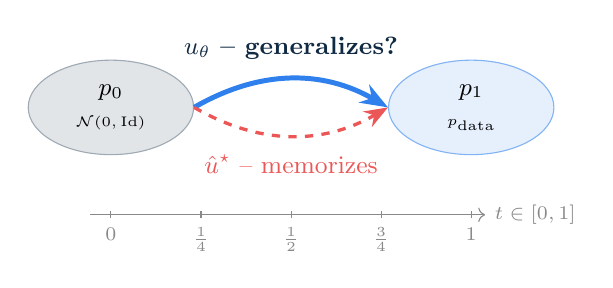
\begin{tikzpicture}[scale=0.88, every node/.style={font=\small}]
        \node[ellipse, fill=TitleColor!12, draw=TitleColor!40,
              minimum width=2.1cm, minimum height=1.2cm, align=center]
              (noise) at (0,0) {$p_0$\\\tiny$\cN(0,\Id)$};
        \node[ellipse, fill=AccentColor!12, draw=AccentColor!60,
              minimum width=2.1cm, minimum height=1.2cm, align=center]
              (data) at (5.2,0) {$p_1$\\\tiny$p_{\mathrm{data}}$};

        \draw[-{Stealth[length=3.5mm]}, line width=1.8pt, AccentColor]
          (noise.east) to[bend left=30]
          node[above=3pt, color=TitleColor, font=\small\bfseries]
          {$u_\theta$ -- generalizes?} (data.west);

        \draw[-{Stealth[length=3mm]}, dashed, line width=1.2pt, RedKO]
          (noise.east) to[bend right=30]
          node[below=3pt, color=RedKO, font=\small]
          {$\hat{u}^\star$ -- memorizes} (data.west);

        \draw[->, TextGray!60, thin] (-0.3,-1.55) -- (5.4,-1.55)
          node[right, font=\scriptsize]{$t\in[0,1]$};
        \foreach \x/\lbl in {0/$0$,1.3/$\tfrac14$,2.6/$\tfrac12$,
                              3.9/$\tfrac34$,5.2/$1$}{
          \draw[TextGray!60,thin] (\x,-1.50)--(\x,-1.60)
            node[below,font=\scriptsize]{\lbl};}
      \end{tikzpicture}
    \end{column}
  \end{columns}
\end{frame}

% ============================================================
\section{Background}
% ============================================================
\begin{frame}{Diffusion Models}
  {Forward SDE, reverse-time sampling, probability-flow ODE}

  \begin{columns}[t]
    \begin{column}{0.48\textwidth}
      \textcolor{TitleColor}{\bfseries Forward process (SDE)}
      \[
        \dd X_t = f(X_t,t)\,\dd t + g(t)\,\dd W_t,
        \quad X_0 \sim p_{\mathrm{data}}
      \]
      Linear SDE: $X_t|X_0\sim\cN(\alpha_t X_0,\sigma_t^2\Id)$

      \vspace{0.35em}
      \textcolor{TitleColor}{\bfseries Reverse-time SDE}
      \[
        \dd\bar{X}_\tau = \!\Big[-f+g^2\,
          \underbrace{\nabla\!\log p_{T-\tau}(\bar{X}_\tau)}_{\text{score}}
        \Big]\dd\tau + g\,\dd\bar{W}_\tau
      \]
      \begin{hlbox}
        \small Score matching loss:
        $\cL_{\mathrm{DSM}} = \E\!\left[
          \left\|s_\theta(\alpha_t x_0+\sigma_t\varepsilon,t)
            +\tfrac{\varepsilon}{\sigma_t}\right\|^2\right]$
      \end{hlbox}
    \end{column}
    \begin{column}{0.48\textwidth}
      \textcolor{TitleColor}{\bfseries Probability-flow ODE \textnormal{\small(bridge to FM)}}
      \[
        \tfrac{\dd}{\dd t}\tilde{X}_t
          = f(\tilde{X}_t,t) - \tfrac{g(t)^2}{2}\nabla\!\log p_t(\tilde{X}_t)
      \]
      \begin{itemize}
        \item Same marginals $p_t$ as the SDE
        \item Fully \textbf{deterministic} -- no noise at inference
        \item Direct bridge to Flow Matching
      \end{itemize}
      \vspace{0.4em}
      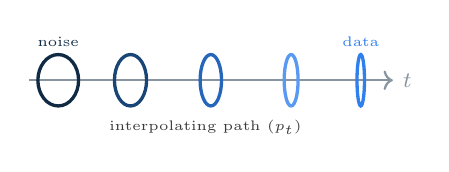
\begin{tikzpicture}[scale=0.68]
        \draw[->,thick,TitleColor!50](-0.3,0)--(6.5,0)node[right,font=\footnotesize]{$t$};
        \foreach \x/\rad/\col in {
            0.25/0.38/TitleColor,
            1.6/0.30/TitleColor!70!AccentColor,
            3.1/0.20/AccentColor!70!TitleColor,
            4.6/0.13/AccentColor!80,
            5.9/0.07/AccentColor}{
          \draw[\col,line width=1.2pt](\x,0) ellipse ({\rad} and {0.48});}
        \node[font=\tiny,TitleColor]at(0.25,0.72){noise};
        \node[font=\tiny,AccentColor]at(5.9,0.72){data};
        \node[font=\tiny,TextGray]at(3,-0.88){interpolating path $(p_t)$};
      \end{tikzpicture}
    \end{column}
  \end{columns}
\end{frame}

\begin{frame}{Flow Matching}
  {Learning a velocity field to transport noise to data}

  \begin{columns}[t]
    \begin{column}{0.48\textwidth}
      \textcolor{TitleColor}{\bfseries The FM framework}

      Learn $u:\R^d\times[0,1]\to\R^d$ such that
      \[
        \dot{x}(t)=u(x(t),t),\quad x(0)\sim\cN(0,\Id)
      \]
      transports $p_0$ to $p_{\mathrm{data}}$.
      Equivalently: $(p_t,u)$ satisfies the
      continuity equation $\partial_t p_t+\nabla\cdot(p_t u)=0$.

      \vspace{0.4em}
      \textcolor{TitleColor}{\bfseries Conditional (Gaussian) path}
      \[
        p_t(\cdot|x_1)=\cN\!\big(tx_1,(1-t)^2\Id\big)
      \]
      with conditional velocity
      $u^{\mathrm{cond}}(x,x_1,t)=\tfrac{x_1-x}{1-t}$.
    \end{column}
    \begin{column}{0.49\textwidth}
      \textcolor{TitleColor}{\bfseries CFM loss}
      \[
        \cL_{\mathrm{CFM}}(\theta)
          = \E\!\left[\norm{u_\theta(x_t,t)-(x_1-x_0)}^2\right]
      \]
      where $x_t=(1-t)x_0+tx_1$.

      \vspace{0.4em}
      \begin{hlbox}[title=Variance decomposition lemma]
        \small For any $A,X$:
        $\E[\|f(X){-}A\|^2]
          = \E[\|f(X){-}\E[A|X]\|^2]
          + \underbrace{\E[\|A{-}\E[A|X]\|^2]}_{\text{indep.\ of }\theta}$\\[3pt]
        $\Rightarrow$ $\cL_{\mathrm{CFM}}$ and the FM loss share the
        \textbf{same gradient and minimizer}:
        \[
          u^\star(x,t)=\E_{z|x,t}\!\big[u^{\mathrm{cond}}(x,z,t)\big].
        \]
      \end{hlbox}
    \end{column}
  \end{columns}
\end{frame}

% ============================================================
\section{Equivalence}
% ============================================================
\begin{frame}{Theoretical Equivalence: FM $\equiv$ Diffusion}
  {Both learn the same probability-flow ODE drift}

  \begin{columns}[c]
    \begin{column}{0.52\textwidth}
      \begin{block}{Theorem 1 \normalfont\small(Lipman et al.\ 2024, Thm.~5.1)}
        Under affine Gaussian paths $x_t=\sigma_t\varepsilon+\alpha_t x_0$,
        the FM optimal velocity equals the PF-ODE drift:
        \[
          \boxed{v^\star(x,t)=f_t\,x-\tfrac{g_t^2}{2}\,\nabla\!\log p_t(x)}
        \]
        where $f_t=\dot\alpha_t/\alpha_t$,
        $g_t^2=2\sigma_t\dot\sigma_t-2f_t\sigma_t^2$.
      \end{block}

      \vspace{0.4em}
      \small\textbf{Proof sketch.} Write $v^\star(x,t)=\E[\dot x_t|x_t=x]$.
      Gaussian posterior identities give
      $\E[\varepsilon|x]=-\sigma_t s$,
      $\E[x_0|x]=\frac{1}{\alpha_t}(x+\sigma_t^2 s)$
      (with $s=\nabla\log p_t$). Substituting and identifying $f_t,g_t$
      yields the result. $\square$

      \vspace{0.4em}
      \textbf{Canonical schedule} $\alpha_t=t,\sigma_t=1-t$:
      $u^{\mathrm{cond}}=x_1-x_0$, the simplest form.
    \end{column}
    \begin{column}{0.44\textwidth}
      \centering
      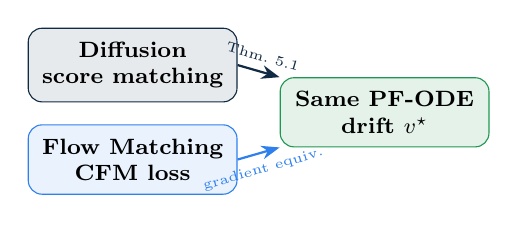
\begin{tikzpicture}[every node/.style={font=\footnotesize}]
        \node[rectangle,rounded corners=5pt,
              fill=TitleColor!10,draw=TitleColor,
              text width=2.3cm,align=center,
              inner sep=5pt,font=\footnotesize\bfseries] (diff) at (0,1.2)
          {Diffusion\\score matching};
        \node[rectangle,rounded corners=5pt,
              fill=AccentColor!10,draw=AccentColor,
              text width=2.3cm,align=center,
              inner sep=5pt,font=\footnotesize\bfseries] (fm) at (0,0)
          {Flow Matching\\CFM loss};
        \node[rectangle,rounded corners=5pt,
              fill=GreenOK!12,draw=GreenOK,
              text width=2.3cm,align=center,
              inner sep=5pt,font=\footnotesize\bfseries] (pf) at (3.2,0.6)
          {Same PF-ODE\\drift $v^\star$};
        \draw[-{Stealth},thick,TitleColor]
          (diff.east)--(pf.north west)
          node[midway,above,sloped,font=\tiny]{Thm.~5.1};
        \draw[-{Stealth},thick,AccentColor]
          (fm.east)--(pf.south west)
          node[midway,below,sloped,font=\tiny]{gradient equiv.};
      \end{tikzpicture}
      \vspace{0.5em}
      \begin{keybox}[title=Key takeaway]
        \small FM and diffusion are \textbf{mathematically
        equivalent}. Generalization \emph{in practice}
        is not explained by equivalence alone.
      \end{keybox}
    \end{column}
  \end{columns}
\end{frame}

% ============================================================
\section{Closed-Form \& Collapse}
% ============================================================
\begin{frame}{Closed-Form Optimal Velocity}
  {An exact formula when training on finite data}

  \begin{columns}[c]
    \begin{column}{0.54\textwidth}
      Replace $p_{\mathrm{data}}$ by
      $\hat{p}=\frac{1}{n}\sum_{i=1}^n\delta_{x^{(i)}}$.

      \begin{block}{Proposition 1 \normalfont\small(Bertrand et al.\ 2025)}
        \[
          \hat{u}^\star(x,t)
            =\sum_{i=1}^n\lambda_i(x,t)\,\frac{x^{(i)}-x}{1-t}
        \]
        $\lambda_i=\mathrm{softmax}\!\big(-\tfrac{\|x-tx^{(j)}\|^2}{2(1-t)^2}\big)_j$
      \end{block}

      \vspace{0.3em}
      \small As $t\to1$: one weight $\lambda_i\to1$ $\Rightarrow$
      $\hat{u}^\star$ points to a \textbf{single training sample}.

      \vspace{0.3em}
      \begin{keybox}[title=The central paradox]
        \small $\hat{u}^\star$ memorizes --- yet $u_\theta$ generalizes.\\[2pt]
        Hypothesis (Vastola): stochasticity of $u^{\mathrm{cond}}$.\\
        \textbf{This paper:} limited capacity. \textcolor{GreenOK}{\bfseries$\checkmark$}
      \end{keybox}
    \end{column}
    \begin{column}{0.42\textwidth}
      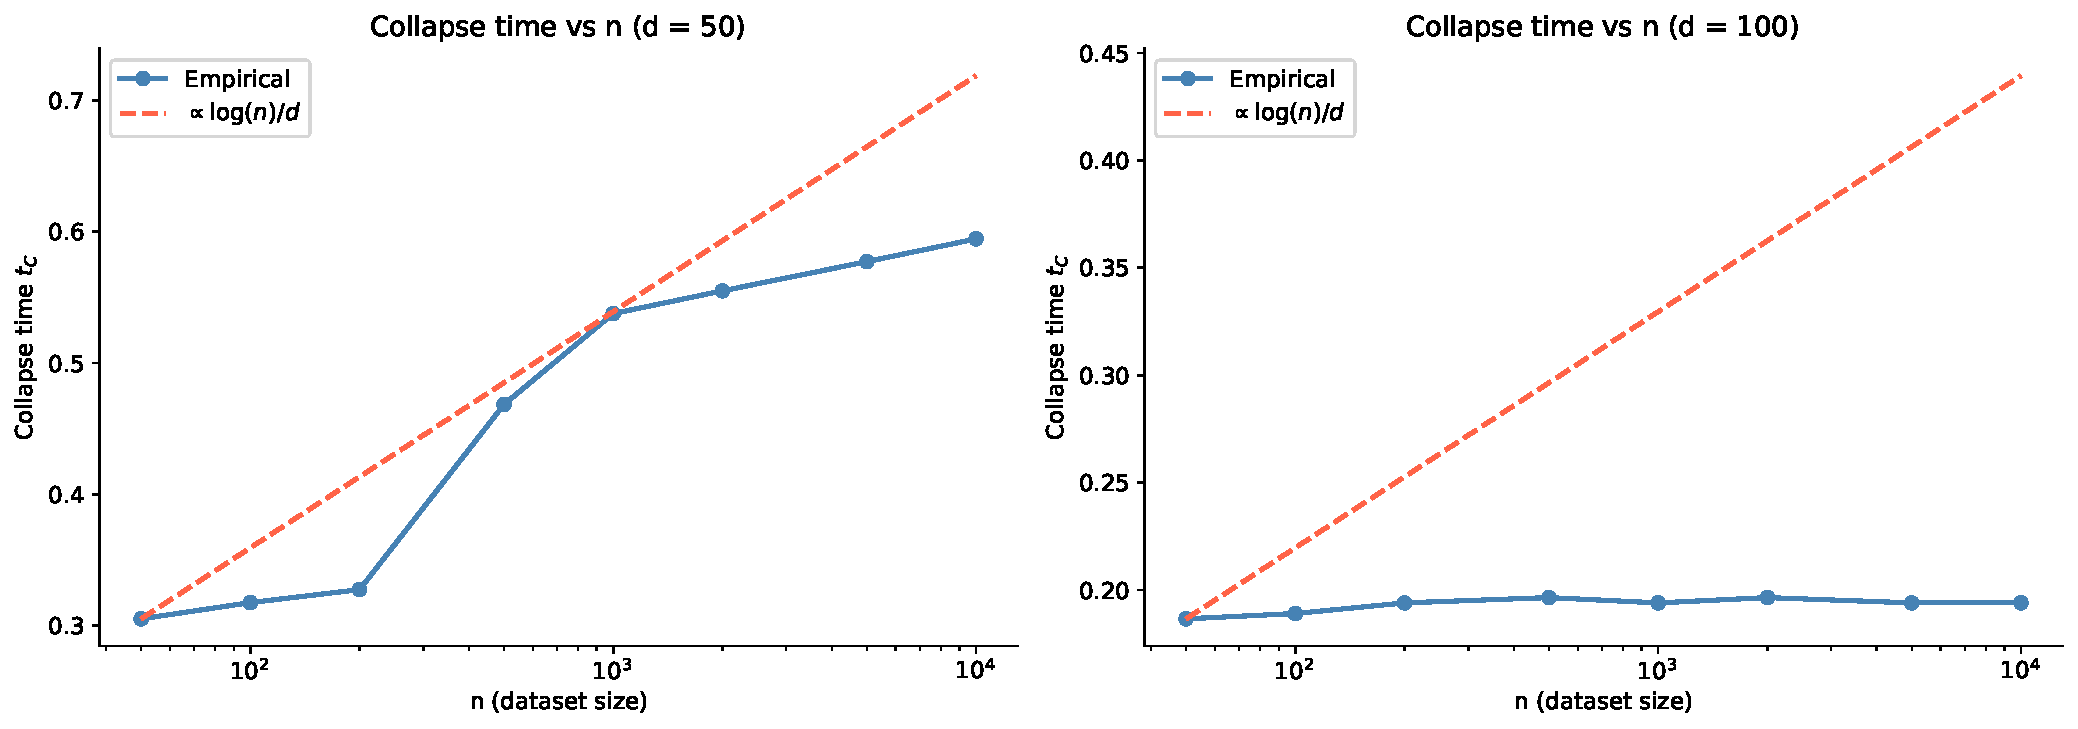
\includegraphics[width=\linewidth]{notebook_1/fig1_collapse_vs_n-2.pdf}
      {\tiny\textcolor{TextGray}{Collapse time $t_C$ vs.\ $n$
        at $d\in\{50,100\}$. Follows $\propto\log(n)/d$ (dashed).}}
    \end{column}
  \end{columns}
\end{frame}

\begin{frame}{Collapse Time: Stochasticity Vanishes in High Dimension}
  {$t_C\sim\mathcal{O}(\log n/d)$: stochastic phase negligible at image resolution}

  \begin{columns}[c]
    \begin{column}{0.46\textwidth}
      \begin{hlbox}[title=Collapse time (Biroli et al.\ 2024)]
        \[
          t_C \;\sim\; \mathcal{O}\!\left(\frac{\log n}{d}\right)
        \]
        \small In high $d$: $t_C\ll1$, stochastic phase
        \textbf{vanishingly short}.
      \end{hlbox}

      \vspace{0.4em}
      \small
      \begin{center}
      \begin{tabular}{lccc}
        \toprule
        Setting & $d$ & $n$ & $t_C$ \\
        \midrule
        2D toy      & 2    & 2000 & 3.8   \\
        $d{=}100$   & 100  & 2000 & 0.075 \\
        CIFAR-10    & 3072 & 50k  & 0.004 \\
        \bottomrule
      \end{tabular}
      \end{center}
    \end{column}
    \begin{column}{0.50\textwidth}
      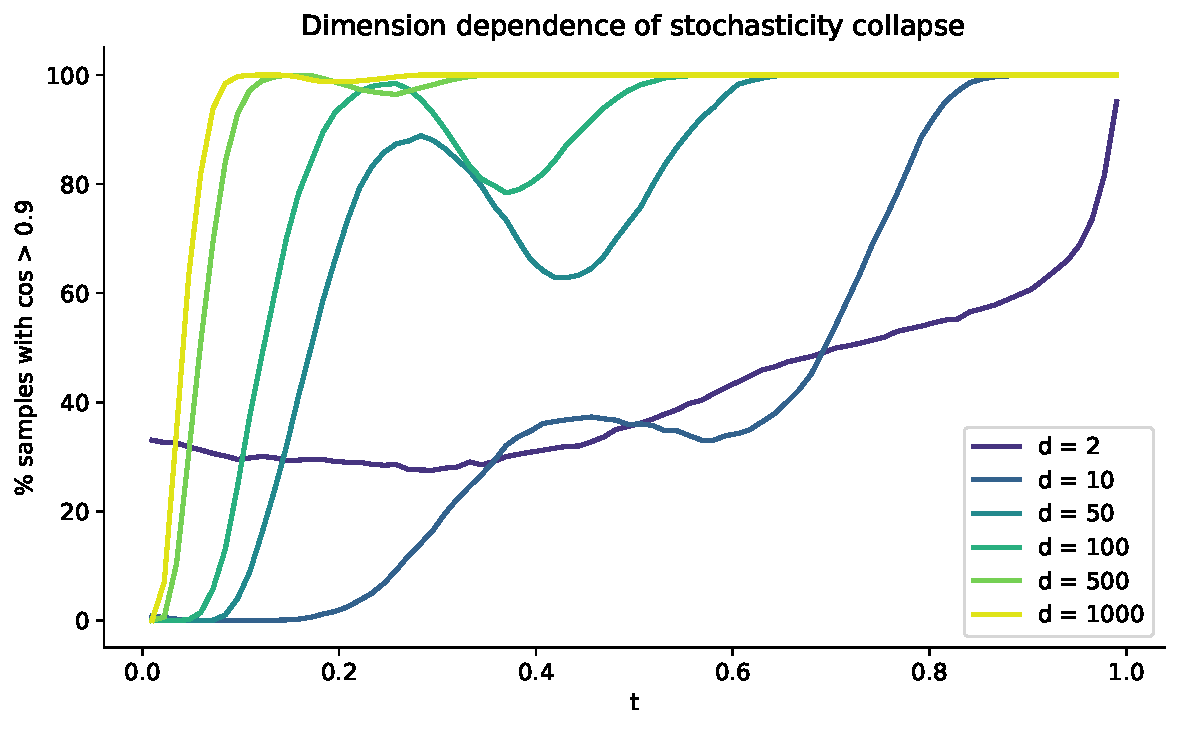
\includegraphics[width=\linewidth]{notebook_1/fig1c_dimension_dependence-2.pdf}
      {\tiny\textcolor{TextGray}{Fraction of pairs with
        $\cos(\hat{u}^\star,u^{\mathrm{cond}})>0.9$ vs.\ $t$,
        $d\in\{2,10,50,100,500,1000\}$, $n=2000$.
        Higher dimension $\Rightarrow$ earlier collapse.}}
    \end{column}
  \end{columns}
\end{frame}

% ============================================================
\section{Experiments}
% ============================================================

% --- Fig 1a: cosine histograms (full width) ---
\begin{frame}{Figure 1a --- Cosine Similarity Histograms}
  {$\cos(\hat{u}^\star,\,u^{\mathrm{cond}})$ at 7 time steps for 3 datasets ($n=5000$)}

  \begin{center}
    \includegraphics[width=0.95\textwidth,height=0.62\textheight,keepaspectratio]%
      {notebook_1/fig1a_cosine_histograms-2.pdf}
  \end{center}
  \vspace{-0.3em}
  \scriptsize\textcolor{TextGray}{%
    Each row: one 2D dataset (moons, rings, Gaussian mix.), each column: one time step.
    Histograms \textbf{concentrate near~1} as $t\to1$ --- softmax collapses to a single training point.
    In high $d$, this collapse occurs at $t<0.1$.}
\end{frame}

% --- Fig 1b+c: collapse time vs Biroli ---
\begin{frame}{Figure 1b\&c --- Collapse Time vs.\ Biroli et al.\ Prediction}
  {Empirical $t_C$ follows $\propto\log(n)/d$ across two orders of magnitude}

  \begin{columns}[c]
    \begin{column}{0.62\textwidth}
      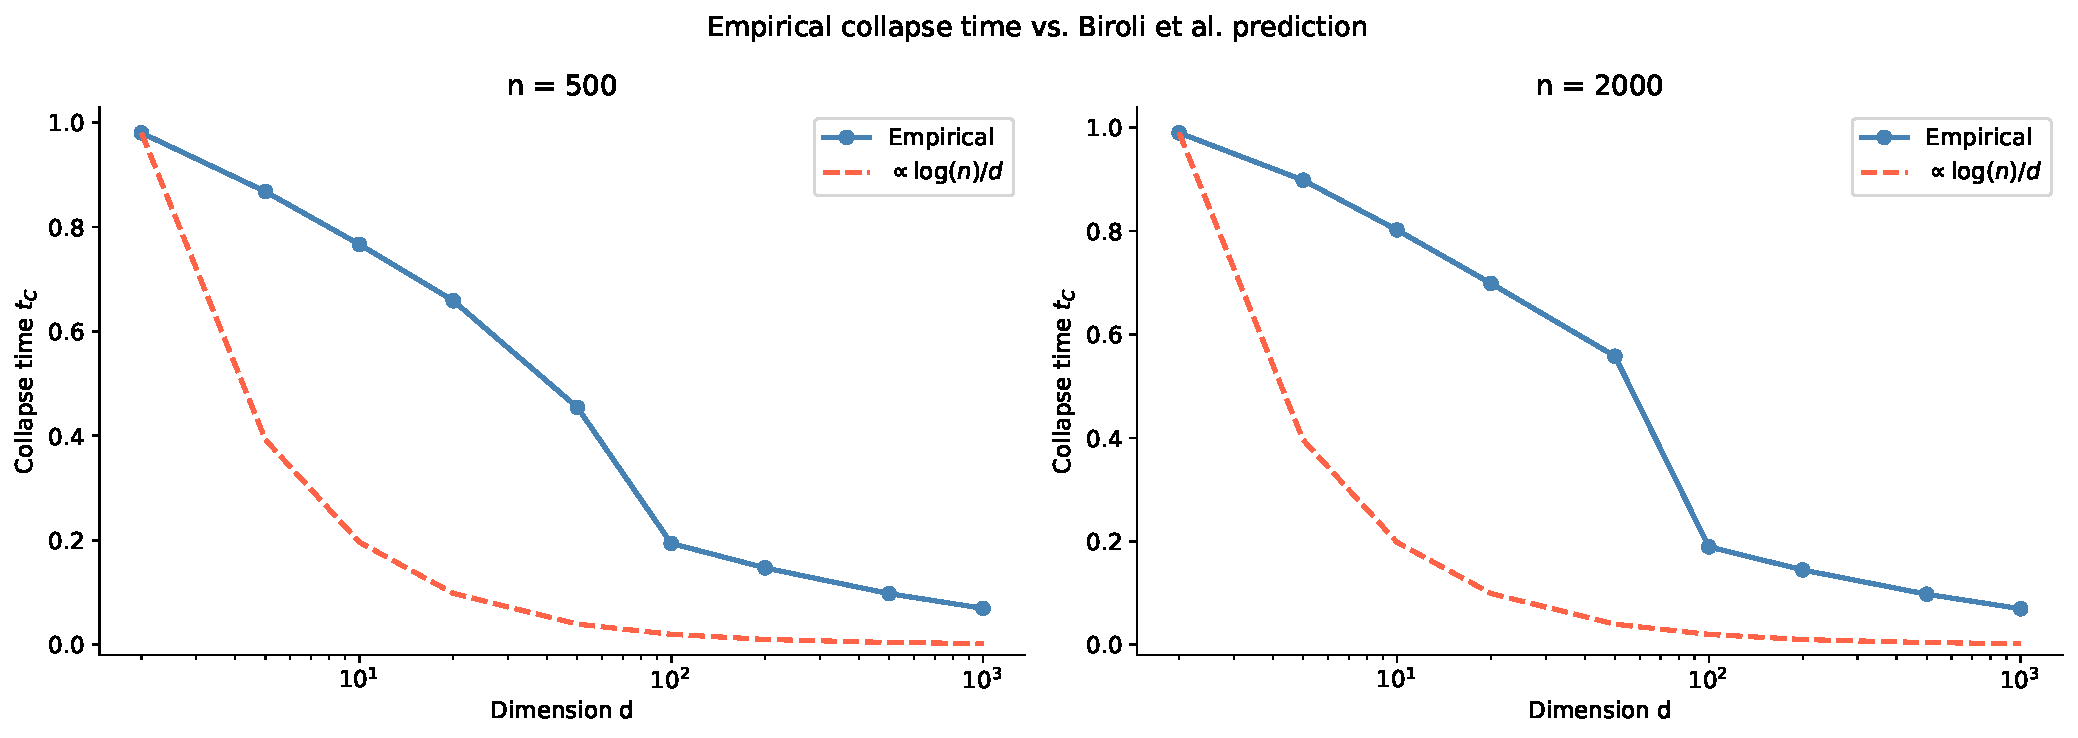
\includegraphics[width=\linewidth]{notebook_1/fig1_collapse_time_vs_theory-2.pdf}
      {\tiny\textcolor{TextGray}{Empirical $t_C$ (blue) vs.\ theoretical $\propto\log(n)/d$
        (dashed red) for $n=500$ and $n=2000$.}}
    \end{column}
    \begin{column}{0.35\textwidth}
      \small
      \textbf{Key findings:}
      \begin{itemize}
        \item Fit is excellent across $d\in[2,\,10^3]$
        \item Both $n=500$ and $n=2000$ follow the same law
        \item The Biroli et al.\ prediction, originally derived
          for \emph{diffusion} models,
          \textbf{transfers to flow matching}
      \end{itemize}
      \vspace{0.4em}
      \begin{resbox}
        \small The stochastic phase covers
        $<4\%$ of the trajectory at $d=3072$
        (CIFAR-10 resolution).
      \end{resbox}
    \end{column}
  \end{columns}
\end{frame}

% --- Fig 2: velocity approximation error + NN distance ---
\begin{frame}{Figure 2 --- Velocity Approximation Failure}
  {The network fails to approximate $\hat{u}^\star$ at two critical time intervals}

  \begin{columns}[c]
    \begin{column}{0.52\textwidth}
      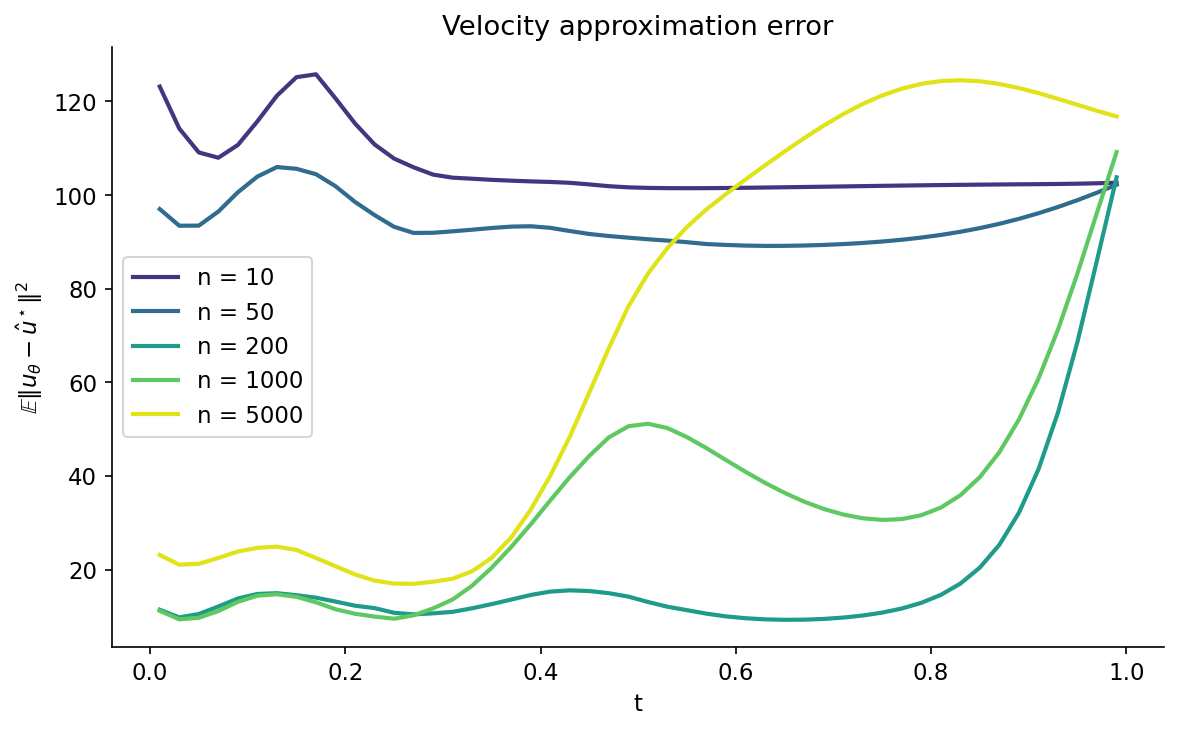
\includegraphics[width=\linewidth]{notebook_2/fig2.png}
      {\tiny\textcolor{TextGray}{$\E\norm{u_\theta-\hat{u}^\star}^2$ vs.\ $t$ for the
        $d=100$ Gaussian mixture, varying $n$.}}
    \end{column}
    \begin{column}{0.45\textwidth}
      \small
      \textbf{Two failure zones:}
      \begin{enumerate}
        \item \textbf{Early bump} ($t\approx0.12$--$0.15$):\\
          stochastic-to-deterministic transition;
          coincides with $t_C$ at $d=100$.
        \item \textbf{Late rise} ($t\to1$):\\
          $\hat{u}^\star$ becomes non-Lipschitz;
          error grows with $n$.
      \end{enumerate}
      \vspace{0.3em}
      \textbf{Causal chain:}\\
      $t<t_C$: $u_\theta\!\approx u^{\mathrm{cond}}\!\neq\!\hat{u}^\star$
      $\Rightarrow$ \textbf{generalization}.\\[3pt]
      $t>t_C$: $u^{\mathrm{cond}}\approx\hat{u}^\star$
      $\Rightarrow$ small error.
      \vspace{0.3em}
      \begin{resbox}
        \scriptsize NN distance $\uparrow$ as $n\uparrow$: large dataset
        forces the model to generalize (capacity bottleneck).
      \end{resbox}
    \end{column}
  \end{columns}
\end{frame}

% --- Fig 3: switching time ---
\begin{frame}{Figure 3 --- Generalization Switching Time}
  {The first $\sim$20\% of the trajectory determines generalization}

  \begin{columns}[c]
    \begin{column}{0.50\textwidth}
      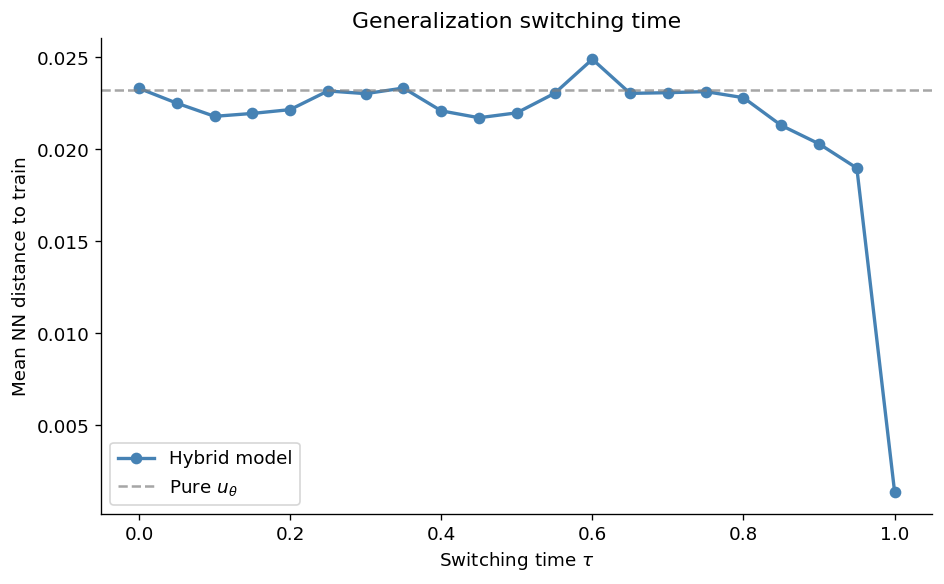
\includegraphics[width=\linewidth]{notebook_3/fig3_hybrid_switching.png}
      {\tiny\textcolor{TextGray}{Mean NN distance vs.\ switching time $\tau$
        for the 2D Gaussian mixture ($n=2000$). Hybrid model:
        follow $\hat{u}^\star$ on $[0,\tau]$, then $u_\theta$ on $[\tau,1]$.}}
    \end{column}
    \begin{column}{0.46\textwidth}
      \small
      \textbf{Setup:} hybrid sampler on 2D Gaussian mix., $n=2000$.

      \vspace{0.4em}
      \textbf{Results:}
      \begin{itemize}
        \item \textbf{Plateau} $\tau\leq0.60$: same NN distance
          as pure $u_\theta$ --- generalization intact
        \item \textbf{Sharp drop} at $\tau\approx0.85$--$0.95$:
          replacing the full trajectory by $\hat{u}^\star$
          collapses generalization
        \item At $\tau=1.0$: pure memorization
      \end{itemize}
      \vspace{0.4em}
      \begin{resbox}[title=Main finding]
        \small Generalization lives where $u_\theta\not\approx\hat{u}^\star$.
        Using $\hat{u}^\star$ in that window eliminates it entirely.
      \end{resbox}
    \end{column}
  \end{columns}
\end{frame}

% --- Sample visualization ---
\begin{frame}{Sample Visualization}
  {From memorization to generalization as $n$ grows}

  \begin{columns}[c]
    \begin{column}{0.58\textwidth}
      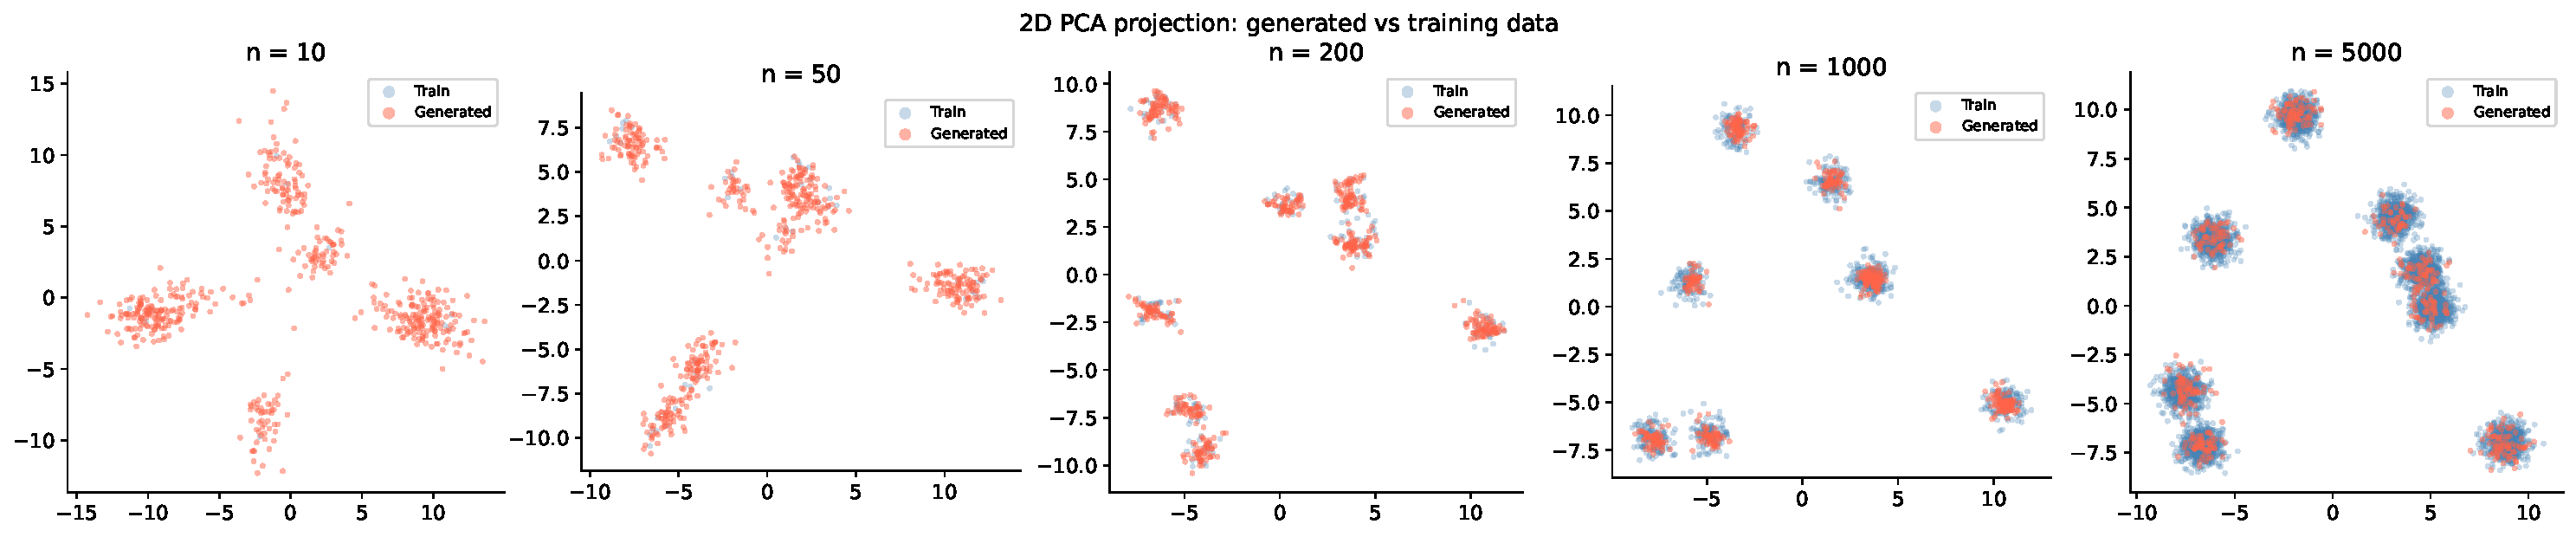
\includegraphics[width=\linewidth]{notebook_2/fig2_scatter_comparison.pdf}
      {\tiny\textcolor{TextGray}{2D PCA projections of generated (red) vs.\ training (blue) samples
        for $n\in\{10,50,200,1000,5000\}$, $d=100$.}}
    \end{column}
    \begin{column}{0.38\textwidth}
      \small
      \begin{itemize}
        \item \textbf{Small $n$} ($n=10$):\\
          generated points cluster \emph{on} training data
          $\Rightarrow$ memorization
        \item \textbf{Large $n$} ($n=5000$):\\
          generated points form a broader distribution
          preserving modal structure $\Rightarrow$ generalization
      \end{itemize}
      \vspace{0.5em}
      \begin{keybox}[title=Interpretation]
        \small As $n$ grows beyond the network capacity,
        $\hat{u}^\star$ becomes too complex to approximate
        $\Rightarrow$ the model \textbf{must} generalize.
      \end{keybox}
    \end{column}
  \end{columns}
\end{frame}

% --- Beyond: geometry + dimension ---
\begin{frame}{Beyond the Paper --- Geometry \& Dimension Scaling}
  {How manifold structure and ambient dimension modulate generalization}

  \begin{columns}[c]
    \begin{column}{0.48\textwidth}
      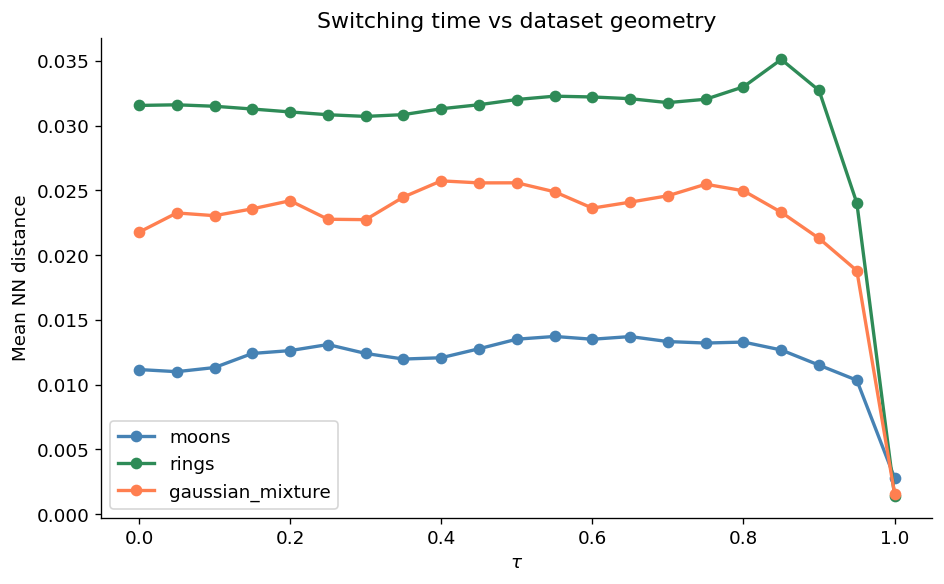
\includegraphics[width=\linewidth]{notebook_3/fig3_geometry_comparison.png}
      {\tiny\textcolor{TextGray}{Switching curves for 3 geometries ($n=2000$).
        Moons (structured, low intrinsic dim) $\to$ lowest NN distance.
        Complexity of $\hat{u}^\star$ depends on the data manifold.}}
    \end{column}
    \begin{column}{0.48\textwidth}
      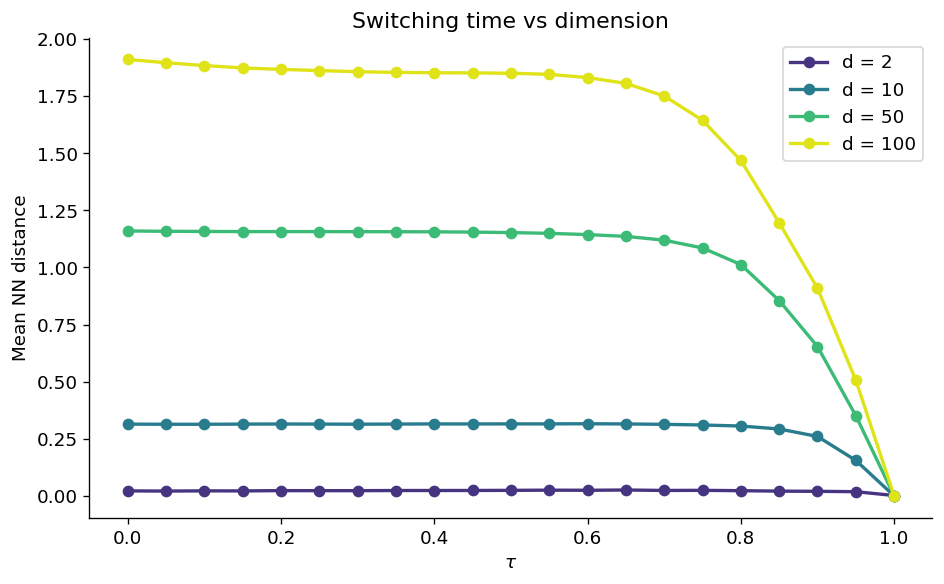
\includegraphics[width=0.49\linewidth]{notebook_3/fig3_dimension_scaling_low.png}%
      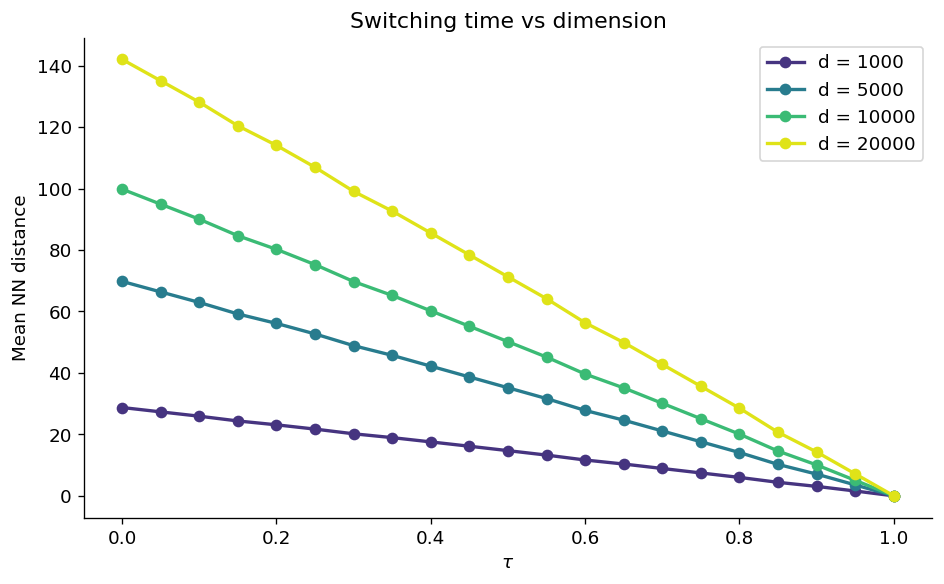
\includegraphics[width=0.49\linewidth]{notebook_3/fig3_dimension_scaling_high.png}
      {\tiny\textcolor{TextGray}{Left: $d\in\{2,10,50,100\}$ --- switching shifts earlier as $d$ grows.
        Right: $d\in\{1000,...,20000\}$ --- curve becomes \emph{flat}: $\hat{u}^\star$
        itself generalizes (mem./gen.\ dichotomy \textbf{vanishes}).}}
      \vspace{0.3em}
      \begin{resbox}
        \small At very high $d$: $t_C\approx\log(n)/d\to0$,
        so $\hat{u}^\star\approx u^{\mathrm{cond}}$ everywhere
        and the closed-form field already generalizes by necessity.
      \end{resbox}
    \end{column}
  \end{columns}
\end{frame}

% --- Beyond: capacity + training ---
\begin{frame}{Beyond the Paper --- Capacity \& Training Duration}
  {Larger/longer-trained models memorize more, not less}

  \begin{columns}[c]
    \begin{column}{0.48\textwidth}
      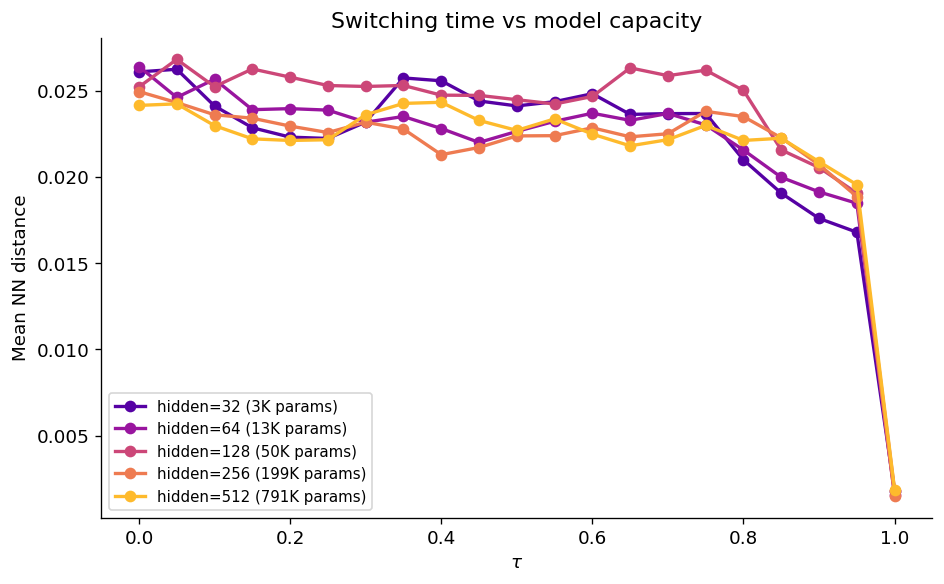
\includegraphics[width=\linewidth]{notebook_3/fig3_capacity.png}
      {\tiny\textcolor{TextGray}{Hidden dim $\in\{32,64,128,256,512\}$
        ($d=2$, Gaussian mix., $n=2000$).
        Larger networks approximate $\hat{u}^\star$ better
        $\Rightarrow$ switching time shifts to smaller $\tau$.
        hidden$=32$: never fully memorizes.}}
    \end{column}
    \begin{column}{0.48\textwidth}
      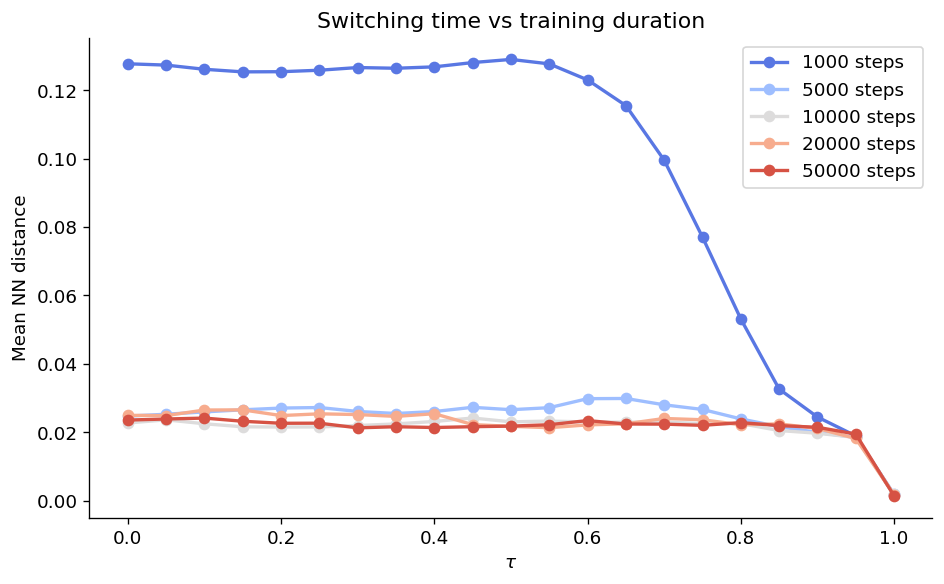
\includegraphics[width=0.95\linewidth]{notebook_3/fig3_training_duration.png}
      {\tiny\textcolor{TextGray}{$\{1k,...,50k\}$ gradient steps.
        Under-trained (1k): flat, strong generalization.
        At 50k: converges; bottleneck is \textbf{capacity}.}}
      \vspace{0.15em}
      \begin{keybox}[title=Consistent message]
        \small More capacity \& training
        $\to$ better $\hat{u}^\star$ approximation
        $\to$ \textbf{more memorization}.\\[1pt]
        \scriptsize Opposite of the prevailing intuition.
      \end{keybox}
    \end{column}
  \end{columns}
\end{frame}

% --- EFM on Fashion-MNIST ---
\begin{frame}{EFM on Fashion-MNIST}
  {Reducing target stochasticity does not improve generalization}

  \begin{columns}[c]
    \begin{column}{0.52\textwidth}
      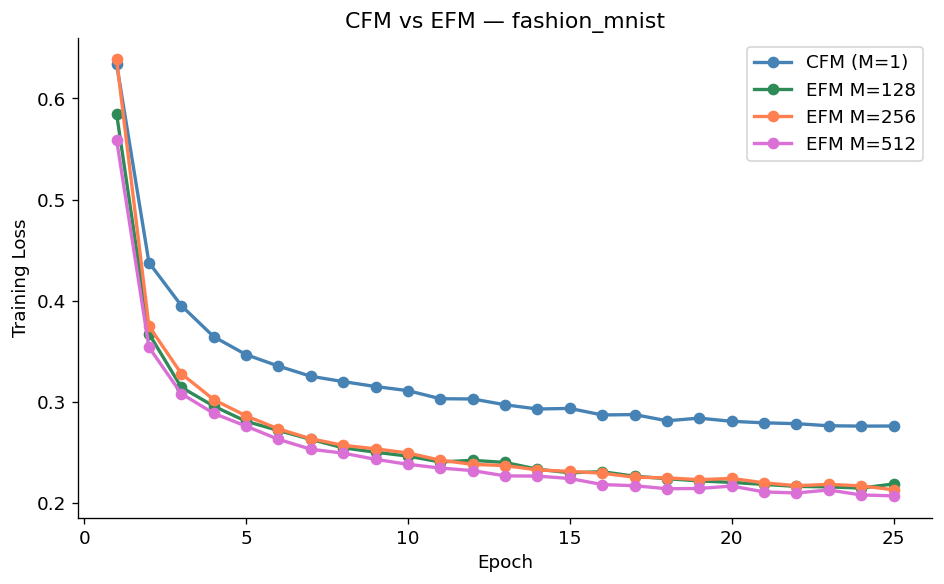
\includegraphics[width=\linewidth]{notebook_4/fig4_training_loss.png}
      {\tiny\textcolor{TextGray}{Training loss (CFM vs.\ EFM for
        $M\in\{128,256,512\}$). EFM achieves significantly lower loss.}}
    \end{column}
    \begin{column}{0.44\textwidth}
      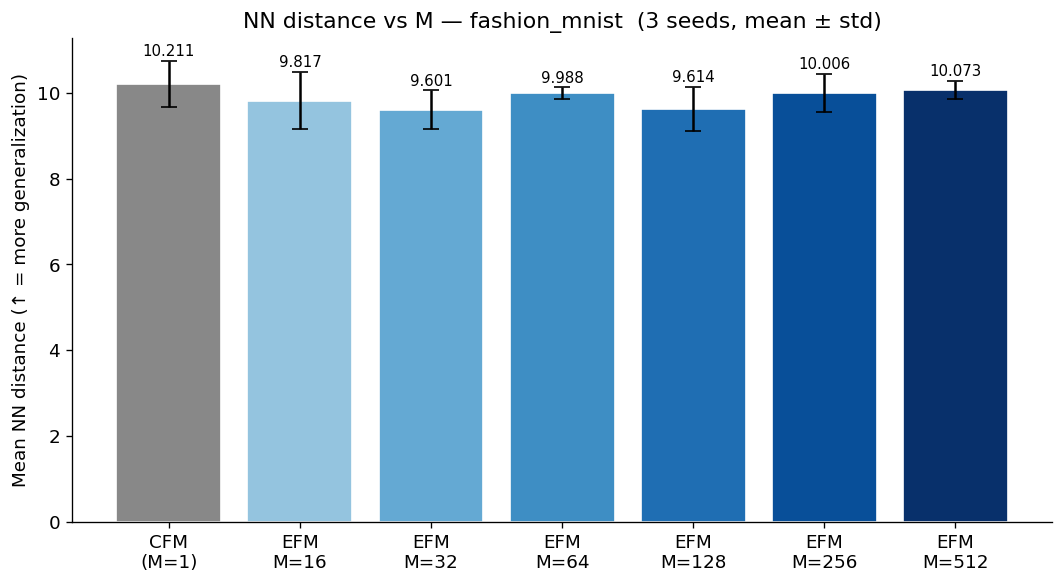
\includegraphics[width=0.95\linewidth]{notebook_4/fig4bis_M_sweep.png}
      {\tiny\textcolor{TextGray}{NN distance vs.\ $M$ (3 seeds): flat.}}
      \vspace{0.2em}
      \small
      \begin{itemize}
        \item EFM replaces $u^{\mathrm{cond}}$ by $\hat{u}^\star_M$
          ($M$ samples per step)
        \item Lower training loss, \textbf{identical generalization}
      \end{itemize}
      \vspace{0.2em}
      \begin{resbox}
        \small Target variance does \textbf{not} drive generalization.\\
        Root cause: \textbf{limited network capacity}.
      \end{resbox}
    \end{column}
  \end{columns}
\end{frame}

% ============================================================
\section{Discussion \& Conclusion}
% ============================================================
\begin{frame}{Discussion}
  {Robust findings and critical perspective}

  \small
  \begin{columns}[t]
    \begin{column}{0.48\textwidth}
      \textcolor{TitleColor}{\bfseries Robust findings}
      \begin{enumerate}
        \item $t_C\sim\log(n)/d$ transfers from
          diffusion to the FM setting
        \item Generalization $\leftrightarrow$ large
          $\E\norm{u_\theta-\hat{u}^\star}^2$ at early/late $t$
        \item More capacity / more training
          $\Rightarrow$ memorization
        \item EFM confirms: noise $\not\Rightarrow$
          generalization
      \end{enumerate}

      \vspace{0.4em}
      \textcolor{TitleColor}{\bfseries Critical perspective}
      \begin{itemize}
        \item \textbf{(i)} Collapse result theoretically expected
          (gradient equiv.\ + measure concentration)
        \item \textbf{(ii)} EFM tension: variance reduction
          only affects the stochastic phase ($<15\%$
          of trajectory at $d=100$)
        \item \textbf{(iii)} True contribution: pinpointing
          \emph{when} generalization occurs via the hybrid model
      \end{itemize}
    \end{column}

    \begin{column}{0.48\textwidth}
      \textcolor{TitleColor}{\bfseries Open questions}
      \begin{itemize}
        \item \textbf{Inductive biases:} U-Net vs.\ MLP
          radically changes $\hat{u}^\star$ approximation
        \item \textbf{Very high $d$:} does $\hat{u}^\star$
          itself generalize at image resolution?
        \item \textbf{Data augmentation} and effective
          complexity of $\hat{u}^\star$
        \item \textbf{LLM memorization:}
          analogous dynamics in token flows?
      \end{itemize}

      \vspace{0.4em}
      \begin{warnbox}
        \small\textbf{Broader implication:}
        Scaling capacity may be at odds with generalization.
        Yet large models generalize on natural images ---
        suggesting \textbf{effective complexity} of $\hat{u}^\star$
        (not raw capacity) is the key quantity.
      \end{warnbox}
    \end{column}
  \end{columns}
\end{frame}

\begin{frame}{Conclusion}

  \begin{columns}[c]
    \begin{column}{0.58\textwidth}
      \begin{block}{Summary}
        \small
        \begin{enumerate}
          \item \textbf{FM $\equiv$ Diffusion:} same PF-ODE drift;
            four prediction targets algebraically equivalent.
          \item \textbf{$\hat{u}^\star$ non-stochastic in high dims:}
            stochastic phase $\sim\log(n)/d$ --- verified on
            toy datasets across two orders of magnitude in $d$.
          \item \textbf{Stochasticity $\not\Rightarrow$ generalization:}
            EFM lowers training loss but not NN distance.
          \item \textbf{Generalization $\Leftarrow$ limited capacity:}
            failure to approximate $\hat{u}^\star$ at early times
            is the true mechanism.
          \item \textbf{Reproduced \& extended:}
            Figs.~1--3 confirmed; ablations on geometry,
            dimension, capacity, training all consistent.
        \end{enumerate}
      \end{block}
    \end{column}

    \begin{column}{0.38\textwidth}
      \centering
      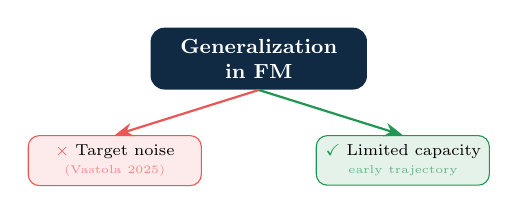
\begin{tikzpicture}[every node/.style={font=\scriptsize},
                          scale=0.82,transform shape]
        \node[rectangle,rounded corners=5pt,
              fill=TitleColor,text=white,
              text width=3.0cm,align=center,
              inner sep=5pt,font=\small\bfseries] (main)
          {Generalization in FM};
        \node[rectangle,rounded corners=4pt,
              fill=RedKO!12,draw=RedKO,
              text width=2.4cm,align=center,inner sep=4pt,
              below left=0.7cm and -0.8cm of main] (wrong)
          {\textcolor{RedKO}{\bfseries$\times$}
           Target noise\\
           \textcolor{RedKO!70}{\tiny(Vastola 2025)}};
        \node[rectangle,rounded corners=4pt,
              fill=GreenOK!12,draw=GreenOK,
              text width=2.4cm,align=center,inner sep=4pt,
              below right=0.7cm and -0.8cm of main] (right)
          {\textcolor{GreenOK}{\bfseries$\checkmark$}
           Limited capacity\\
           \textcolor{GreenOK!70}{\tiny early trajectory}};
        \draw[-{Stealth},RedKO,thick](main.south)--(wrong.north);
        \draw[-{Stealth},GreenOK,thick](main.south)--(right.north);
      \end{tikzpicture}
      \vspace{0.6em}
      {\scriptsize\textcolor{TextGray}{All experiments on a single
        Google Colab T4 GPU in $<$30~min/notebook.}}
    \end{column}
  \end{columns}
\end{frame}

% ============================================================
%  APPENDIX
% ============================================================
\appendix

\begin{frame}{References}
  \footnotesize
  \begin{enumerate}
    \item \textbf{Bertrand, Gagneux, Massias, Emonet.}
      \textit{On the closed-form of flow matching.} NeurIPS 2025.
    \item \textbf{Biroli, Bonnaire, de Bortoli, M{\'e}zard.}
      \textit{Dynamical regimes of diffusion models.}
      Nature Comm.\ 15(1):9957, 2024.
    \item \textbf{Lipman, Chen, Ben-Hamu, Nickel, Le.}
      \textit{Flow matching for generative modeling.} ICLR 2023.
    \item \textbf{Lipman et al.}
      \textit{Flow matching guide and code.} arXiv:2412.06264, 2024.
    \item \textbf{Liu, Gong, Liu.}
      \textit{Flow straight and fast: rectified flow.} ICLR 2023.
    \item \textbf{Albergo, Vanden-Eijnden.}
      \textit{Building normalizing flows with stochastic interpolants.}
      ICLR 2023.
    \item \textbf{Ho, Jain, Abbeel.}
      \textit{Denoising diffusion probabilistic models.} NeurIPS 2020.
    \item \textbf{Song et al.}
      \textit{Score-based generative modeling through SDEs.} ICLR 2021.
    \item \textbf{Vastola.}
      \textit{Generalization through variance.} ICLR 2025.
    \item \textbf{Gao, Li.}
      \textit{How do FM models memorize and generalize?}
      arXiv:2410.23594, 2024.
  \end{enumerate}
\end{frame}

% ────────────────────────────────────────────────────────────
\begin{frame}{Appendix A --- Proof Sketch of Theorem 1}
  {FM optimal velocity $=$ PF-ODE drift}

  Under affine Gaussian paths $x_t=\sigma_t\varepsilon+\alpha_t x_0$,
  write $\dot x_t=\sigma_t'\varepsilon+\alpha_t'x_0$.

  \medskip
  \textbf{Step 1.}
  $v^\star(x,t)=\E[\dot x_t|x_t=x]
    =\sigma_t'\E[\varepsilon|x]+\alpha_t'\E[x_0|x]$.

  \medskip
  \textbf{Step 2.} Gaussian posterior mean identities
  (setting $s=\nabla\log p_t$):
  \[
    \E[\varepsilon|x]=-\sigma_t s(x,t), \qquad
    \E[x_0|x]=\tfrac{1}{\alpha_t}(x+\sigma_t^2 s(x,t)).
  \]

  \textbf{Step 3.} Substituting:
  \[
    v^\star(x,t)
      =\frac{\dot\alpha_t}{\alpha_t}\,x
      +\!\left(\frac{\dot\alpha_t}{\alpha_t}\sigma_t^2
               -\dot\sigma_t\sigma_t\right)s(x,t).
  \]

  \textbf{Step 4.} Setting $f_t=\dot\alpha_t/\alpha_t$ and
  $g_t^2=2\sigma_t\dot\sigma_t-2f_t\sigma_t^2$ gives
  $(\cdots)=-g_t^2/2$, so:
  \[
    \boxed{v^\star(x,t)=f_t\,x-\tfrac{g_t^2}{2}\,\nabla\log p_t(x)}
    \qquad\square
  \]
\end{frame}

% ────────────────────────────────────────────────────────────
\begin{frame}{Appendix B --- EFM Algorithm}
  {Eliminating stochasticity from the training target}

  \textbf{EFM loss:} replace $u^{\mathrm{cond}}$ by a Monte Carlo
  estimate $\hat{u}^\star_M$ with $M$ samples:
  \[
    \cL_{\mathrm{EFM}}(\theta)
      = \E\!\left[\norm{u_\theta(x_t,t)-\hat{u}^\star_M(x_t,t)}^2\right]
  \]
  where $b^{(1)}:=x_1$ (the conditioning point) and
  \[
    \hat{u}^\star_M(x,t)
      =\sum_{j=1}^M\frac{b^{(j)}-x}{1-t}
       \cdot\mathrm{softmax}\!\left(
         -\frac{\|x-tb^{(k)}\|^2}{2(1-t)^2}
       \right)_{\!k,j}.
  \]

  \begin{columns}[t]
    \begin{column}{0.48\textwidth}
      \textbf{Key property:} including $x_1$ as $b^{(1)}$
      makes $\hat{u}^\star_M$ \emph{unbiased}
      (Prop.~2, Bertrand et al.) with lower variance.
      As $M\to\infty$: $\hat{u}^\star_M\to\hat{u}^\star$ pointwise.
    \end{column}
    \begin{column}{0.48\textwidth}
      \textbf{Fashion-MNIST:} EFM achieves strictly lower
      training loss but \textbf{identical NN distances}
      across all $M\in\{1,...,512\}$.
      This definitively rules out stochasticity as a
      driver of generalization.
    \end{column}
  \end{columns}
\end{frame}

% ────────────────────────────────────────────────────────────
\begin{frame}{Appendix C --- Collapse Time Derivation}
  {Why $t_C\sim\mathcal{O}(\log n/d)$}

  \textbf{Softmax dominance condition:}
  weight $\lambda_{i^\star}$ dominates when the gap in the exponent
  exceeds $\log n$, i.e.\
  $\frac{\|x_t-tx^{(i^\star)}\|^2-\|x_t-tx^{(j)}\|^2}{2(1-t)^2}\gg\log n$
  for all $j\neq i^\star$.

  \medskip
  \textbf{Scaling of squared distances:}
  For i.i.d.\ Gaussian data in $\R^d$, pairwise distances concentrate
  around $\sim d$ (law of large numbers).
  Along $x_t=(1-t)x_0+tx_1$, the nearest-neighbour gap scales
  as $\sim d\cdot t^2$.
  Solving gap $\sim d\cdot t_C=\log n$ gives:
  \[
    \boxed{t_C\;\approx\;\frac{\log n}{d}}
  \]

  \textbf{CIFAR-10 example} ($d=3072$, $n=50\,000$):
  \[
    t_C\approx\frac{\log 50000}{3072}\approx0.036
    \quad\Rightarrow\quad \text{stochastic phase} < 4\%.
  \]

  \begin{resbox}
    \small The Biroli et al.\ result, proved for diffusion models
    via a careful SDE analysis, holds empirically for FM --- confirmed
    across two orders of magnitude in $d$ on our toy datasets.
  \end{resbox}
\end{frame}

% ────────────────────────────────────────────────────────────
\begin{frame}{Appendix D --- Ablation Summary}

  \small
  \begin{center}
    \renewcommand{\arraystretch}{1.20}
    \begin{tabular}{p{2.6cm}p{1.8cm}p{2.6cm}p{4.6cm}}
      \toprule
      \textbf{Variable} & \textbf{Effect} & \textbf{Mechanism}
        & \textbf{Interpretation} \\
      \midrule
      $\uparrow$ dim.\ $d$
        & $\tau^\star$ $\downarrow$
        & $t_C\propto1/d$
        & non-stochastic regime starts earlier \\
      $\uparrow$ size $n$
        & stable
        & capacity bottleneck
        & same failure zone \\
      $\uparrow$ capacity
        & $\tau^\star$ $\downarrow$
        & better $\hat{u}^\star$ approx.
        & failure window shrinks \\
      $\uparrow$ training
        & $\tau^\star$ $\downarrow$
        & better $\hat{u}^\star$ approx.
        & bottleneck: capacity not opt. \\
      Geometry
        & varies
        & $\hat{u}^\star$ complexity
        & moons $\to$ earliest switching \\
      $\uparrow M$ (EFM)
        & no change
        & noise $\not\to$ gen.
        & central claim confirmed \\
      $d\geq1000$
        & flat curve
        & $\hat{u}^\star$ generalizes
        & dichotomy vanishes \\
      \bottomrule
    \end{tabular}
  \end{center}

  \vspace{0.3em}
  \begin{resbox}
    \small\textbf{All ablations} consistently support:
    generalization $\Leftrightarrow$ poor $\hat{u}^\star$ approximation
    at early times, driven by limited network expressiveness.
  \end{resbox}
\end{frame}

\end{document}
